% 问题一第三小问：领域配比与交叉熵损失的定量关系
% 数值来源及数据角色见 docs/problem/q1-s03-data-model-guide.md。
\section{问题一：领域配比与交叉熵损失的定量关系}
\label{sec:q13}

\subsection{数据角色与前两问的衔接}

第一小问建立了以 $A_1$ 为拟合参照的质量分数 $Q_i$，第二小问进一步把多指标信号的相对高低组合标记为候选冲突，并区分测量分歧、属性权衡和适用性疑点。第三小问的直接目标不同：在 17 个领域配比满足单纯形约束的条件下，建立配比向量与 13 个交叉熵验证损失之间的定量关系。因而，本节把配比作为主解释变量，把第一、二小问得到的质量信息只作为可选增量或解释约束；质量分数不替代配比主模型，也不被解释为交叉熵损失的独立因果变量。

数据表按题目编号分成六个角色。$A_4/A_5$ 共 512 行、规模标签为 $1\,\mathrm{M}$，用于模型拟合、交叉验证和候选模型选择；$A_6/A_7$ 共 256 行、规模同为 $1\,\mathrm{M}$，用于同尺度外部验证；$A_8/A_9$ 共 256 行、规模为 $60\,\mathrm{M}$，其配方与 $A_6/A_7$ 逐行相同，可用于配对规模差异；$A_{10}/A_{11}$ 共 64 行、规模为 $1\,\mathrm{B}$，同时发生规模与配方变化，只能作为回顾性迁移诊断；$A_{12}/A_{13}$ 和 $A_{14}/A_{15}$ 各 63 行，分别为 $10\,\mathrm{B}$ 和 $70\,\mathrm{B}$ 的给定估算表，主要用于外推审计。总计 1,214 行，其中 $A_{12}/A_{14}$ 的配方是 $A_4/A_5$ 中前 63 个配方的精确子集，因此这两组数据是已见配方上的规模外推，而不是新的配方外推。

\begin{table}[htbp]
  \centering
  \caption{第三小问数据的拟合、验证与外推角色}
  \label{tab:q13-data-role}
  \renewcommand{\arraystretch}{1.12}
  \begin{tabular}{lrrll}
    \toprule
    数据表 & 行数 & 规模 & 配方关系 & 本节用途 \\
    \midrule
    $A_4/A_5$ & 512 & $1\,\mathrm{M}$ & 训练配方 & 拟合、交叉验证、模型选择 \\
    $A_6/A_7$ & 256 & $1\,\mathrm{M}$ & 新配方 & 同尺度外部验证 \\
    $A_8/A_9$ & 256 & $60\,\mathrm{M}$ & 与 $A_6/A_7$ 同配方 & 配对规模诊断 \\
    $A_{10}/A_{11}$ & 64 & $1\,\mathrm{B}$ & 规模与配方均变化 & 回顾性迁移诊断 \\
    $A_{12}/A_{13}$ & 63 & $10\,\mathrm{B}$ & 已见配方估算 & 外推审计 \\
    $A_{14}/A_{15}$ & 63 & $70\,\mathrm{B}$ & 与 $A_{12}/A_{13}$ 同配方 & 外推审计 \\
    \bottomrule
  \end{tabular}
\end{table}

\subsection{单纯形表示与评价口径}

记第 $r$ 行的 17 域配比为 $\boldsymbol p_r=(p_{r1},\ldots,p_{r,17})$。预处理先检查非负性，再按行归一化到
\begin{equation}
  \Delta_{17}=\left\{\boldsymbol p\in\mathbb R_+^{17}:\sum_{i=1}^{17}p_i=1\right\}.
  \label{eq:q13-simplex}
\end{equation}
由于配比数据含零值，采用乘法零替换，令零替换常数为 $\varepsilon=10^{-4}$，再以 Helmert 对数比变换得到 16 维坐标
\begin{equation}
  \boldsymbol z_r=\operatorname{ilr}_{\mathrm{Helmert}}\!\left(\boldsymbol p_r^{(\varepsilon)}\right)\in\mathbb R^{16}.
  \label{eq:q13-ilr}
\end{equation}
该表示保留单纯形的相对信息，避免直接将 17 个和为 1 的分量作为相互独立的自变量。零替换参数和坐标基会影响数值系数，因此后文的系数只用于当前协议下的预测与有限替代分析，不作无条件的领域因果解释。

设 $y_{rj}$ 为第 $r$ 行第 $j$ 个交叉熵损失，$j=1,\ldots,13$。主指标采用 pooled RMSE 和 pooled MAE，即分别在全部样本—目标残差 $e_{rj}=\hat y_{rj}-y_{rj}$ 上计算
\begin{equation}
  \operatorname{RMSE}=\sqrt{\frac{1}{13n}\sum_{r,j}e_{rj}^2},\qquad
  \operatorname{MAE}=\frac{1}{13n}\sum_{r,j}|e_{rj}|.
  \label{eq:q13-metrics}
\end{equation}
同时报告 13 个目标的平均 $R^2$ 作为诊断。先对 13 个损失求行均值再计算误差会产生域间抵消，故不与 pooled 指标混合排名。

\subsection{配比—损失模型与模型选择}

首先用训练集目标均值作为无配比信息的参照。可解释基线为逐目标 ILR 线性 Ridge
\begin{equation}
  \widehat y_{rj}^{\mathrm{lin}}=a_j+\boldsymbol b_j^{\mathsf T}\boldsymbol z_r,
  \label{eq:q13-linear}
\end{equation}
并以二阶多项式 Ridge 检查组合项带来的非线性预测增量：
\begin{equation}
  \widehat y_{rj}^{\mathrm{quad}}
  =a_j+\boldsymbol b_j^{\mathsf T}\boldsymbol z_r
   +\boldsymbol z_r^{\mathsf T}\boldsymbol C_j\boldsymbol z_r.
  \label{eq:q13-quadratic}
\end{equation}
此外，将 PLS 和浅层 GBDT 作为降维与树模型参照。所有模型仅在 $A_4/A_5$ 上进行 3 个随机种子、5 折重复交叉验证，超参数由该交叉验证选择；冻结后的模型在 $A_6/A_7$ 上做同尺度外部验证。$A_8$--$A_{15}$ 不参与模型选择。

\begin{table}[htbp]
  \centering
  \caption{候选模型在 $A_4/A_5$ 重复交叉验证和 $A_6/A_7$ 同尺度外部验证上的 pooled 指标}
  \label{tab:q13-model-benchmark}
  \renewcommand{\arraystretch}{1.12}
  \begin{tabular}{lrrrrr}
    \toprule
    模型 & CV RMSE & CV MAE & 验证 RMSE & 验证 MAE & 验证 $R^2$ \\
    \midrule
    均值基线 & 0.8246$\pm$0.0238 & 0.6442$\pm$0.0195 & 0.7798 & 0.6193 & $-0.0125$ \\
    ILR-OLS & 0.3971$\pm$0.0212 & 0.2875$\pm$0.0137 & 0.3472 & 0.2633 & 0.7635 \\
    ILR-Ridge & 0.3971$\pm$0.0215 & 0.2873$\pm$0.0137 & 0.3464 & 0.2626 & 0.7649 \\
    PLS & 0.4674$\pm$0.0223 & 0.3476$\pm$0.0145 & 0.4096 & 0.3133 & 0.6464 \\
    \textbf{二阶 Ridge} & \textbf{0.3411$\pm$0.0243} & \textbf{0.2383$\pm$0.0134} & \textbf{0.2840} & \textbf{0.2019} & \textbf{0.8661} \\
    浅层 GBDT & 0.3528$\pm$0.0186 & 0.2539$\pm$0.0116 & 0.3066 & 0.2307 & 0.8192 \\
    \bottomrule
  \end{tabular}
  \vspace{1mm}
  \parbox{0.95\linewidth}{\footnotesize 注：CV 数值为选定超参数下 15 个折—种子组合的均值$\pm$标准差；验证指标为 $A_6/A_7$ 全部样本与 13 个目标上的 pooled 指标。}
\end{table}

二阶 Ridge 在当前候选集合中同时取得最低的交叉验证 RMSE/MAE 和最低的 $A_6/A_7$ 外部误差，浅层 GBDT 次之。相对于均值基线，二阶 Ridge 将同尺度 pooled MAE 从 0.6193 降至 0.2019。该结果支持“配比包含可预测的损失差异”，但不支持把二阶模型的 152 个交互特征逐项解释为稳定的协同或因果效应；组合效应需在单纯形内部做有限替代并进行稳定性审计。

\begin{figure}[htbp]
  \centering
  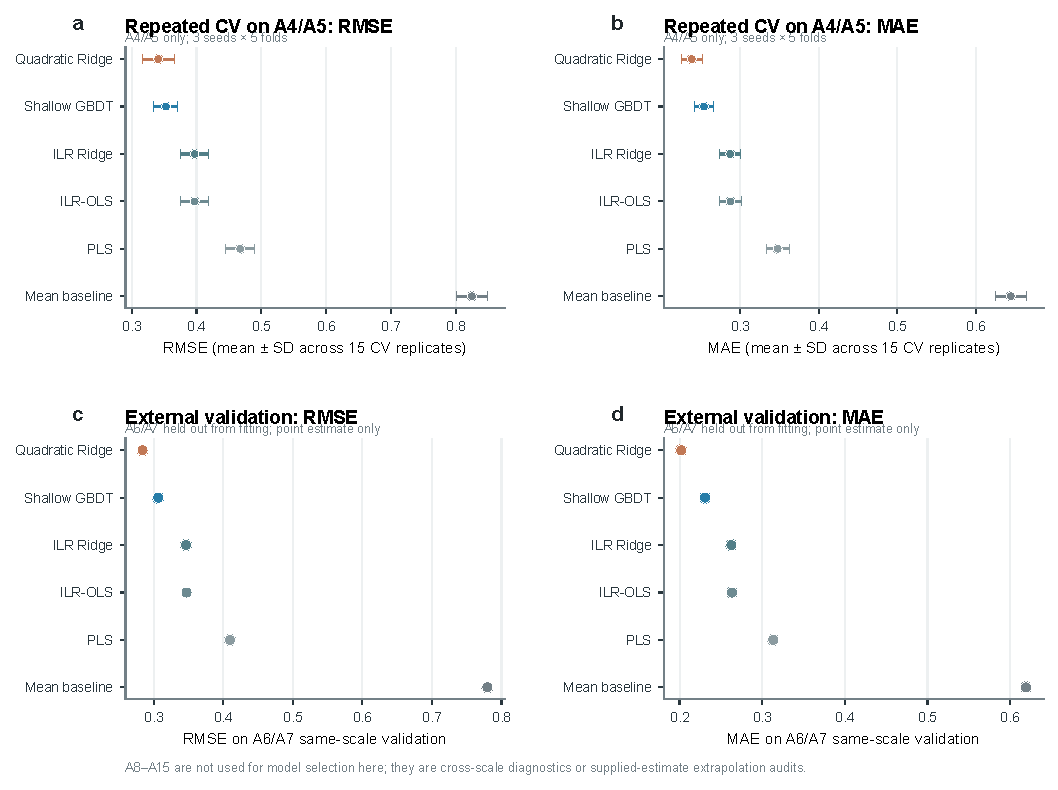
\includegraphics[width=\linewidth]{figures/q1-mixture-loss/Figure5_Q1_S03_model_selection_validation.pdf}
  \caption{配比模型候选与同尺度外部验证。a,b，$A_4/A_5$ 上选定超参数的 3 个随机种子、5 折重复交叉验证 RMSE 和 MAE；c,d，冻结训练集拟合后在 $A_6/A_7$ 上的 pooled RMSE 和 MAE。$A_8$--$A_{15}$ 未参与模型选择。}
  \label{fig:q13-model-benchmark}
\end{figure}

\subsection{规模效应必须与配方迁移分离}

由于 $A_6/A_7$ 与 $A_8/A_9$ 的配方矩阵完全相同，可以定义同一配方的配对差
\begin{equation}
  \Delta_j(\boldsymbol p)=L_j(\boldsymbol p,1\,\mathrm{M})-L_j(\boldsymbol p,60\,\mathrm{M}).
  \label{eq:q13-paired-scale}
\end{equation}
256 个配对在 13 个目标上均表现为低规模损失较高，平均下降量为 $1.4594$；换算为对数规模区间的描述性斜率约为每十进制 $0.8207$。这条证据只说明在该配方集合和该规模区间存在一致的规模差异，不直接给出可迁移到任意配方、任意规模的统一规模系数。

这组配对还给出了不含规模项的 $\widehat L=f(\boldsymbol p)$ 模型的不可避免误差下界：同一配方在两个规模上的共享预测至少产生半差值误差，对 $A_6/A_8$ 的平均 Loss 而言，MAE 和 RMSE 下界分别约为 $0.7297$ 和 $0.7677$。因此，跨规模误差的主要来源不能被重新归因于配比本身，模型至少需要把规模标签或规模条件项显式纳入迁移分析。

将 $A_6/A_7$ 与 $A_{10}/A_{11}$ 直接比较时，规模从 $1\,\mathrm{M}$ 变为 $1\,\mathrm{B}$ 的同时，17 个领域的配比也发生变化。例如 Pile-CC 占比增加约 0.118，而 GitHub 占比减少约 0.027，因此该对比是“规模+配方迁移”而不是纯规模实验。图~\ref{fig:q13-core} 将配对规模差、17 域配比变化、各表 13 域平均损失和旧质量代理诊断放在同一框架中；图中 M1/B1 只用于历史工程路线的误差诊断，不能与表~\ref{tab:q13-model-benchmark} 的 composition-only 二阶 Ridge 直接排名。

\begin{figure}[htbp]
  \centering
  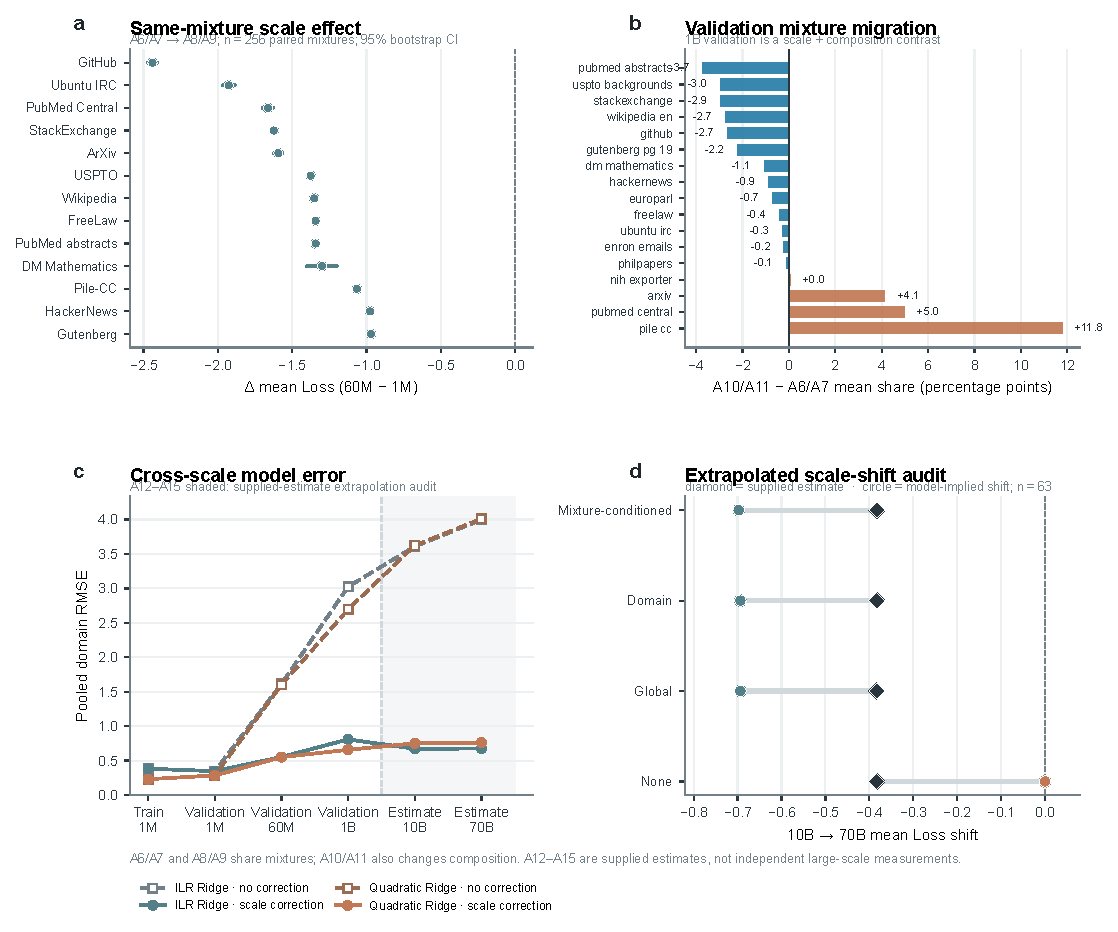
\includegraphics[width=\linewidth]{figures/q1-mixture-loss/Figure3_Q1_S03_core_analysis.pdf}
  \caption{同配方规模效应与配方迁移。a，$A_6/A_7\rightarrow A_8/A_9$ 的配对域级损失变化（点为均值，线为 95\% bootstrap 区间）；b，$A_{10}/A_{11}$ 相对 $A_6/A_7$ 的 17 域配比变化；c，各数据表的 13 域平均损失；d，历史 M1 相对 B1 的域级误差诊断。$A_{10}/A_{11}$ 同时改变规模与配方，$A_{12}$--$A_{15}$ 的损失为给定估计值。}
  \label{fig:q13-core}
\end{figure}

进一步，$A_{12}/A_{14}$ 的相同配方提供了高规模区间的配对审计。其 $10\,\mathrm{B}\rightarrow70\,\mathrm{B}$ 平均损失下降仅为 $0.3829$，按对数区间换算约为每十进制 $0.4531$，低于 $1\,\mathrm{M}\rightarrow60\,\mathrm{M}$ 的 $0.8207$。若把低规模下降量按对数间隔直接转移到高规模区间，得到的平均下降为 $0.6936$，比给定估计值高出 $0.3107$，13 个目标均出现高估。因而，配比效应必须通过同配方配对和配方迁移分析分离，不能用两个规模表的总差异直接当作配比效应或全局规模系数。

\subsection{配方支持域与迁移边界}

为了检查跨表配方是否离开训练支持域，对配比作带 $\varepsilon$ 的 CLR 诊断，并计算各样本到 $A_4/A_5$ 配方集合的最近 Aitchison 距离。主图采用 $\varepsilon=10^{-4}$，同时检查 $10^{-6}$ 和 $10^{-5}$。在该诊断下，$A_6/A_7$ 和 $A_8/A_9$ 的最近训练距离均值约为 8.45，$A_{10}/A_{11}$ 约为 7.83；$A_{12}/A_{14}$ 的距离为 0，因为其配方是训练配方的精确子集。距离的绝对数值随零替换参数变化，因此图~\ref{fig:q13-support} 只用于描述支持域和误差随迁移距离的关系，不把二维投影或距离本身解释为因果证据。

\begin{figure}[htbp]
  \centering
  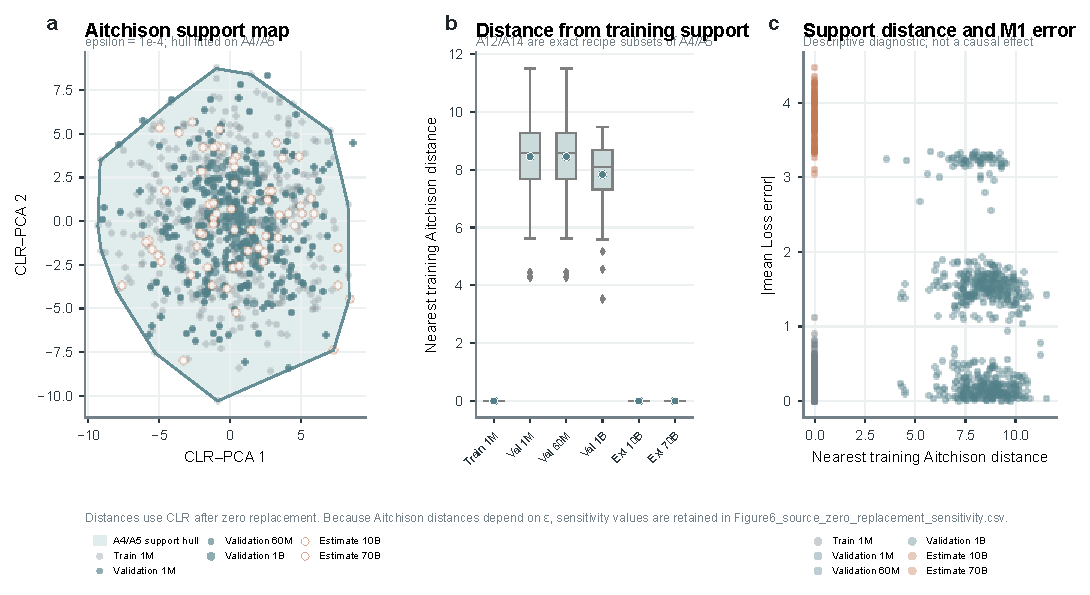
\includegraphics[width=\linewidth]{figures/q1-mixture-loss/Figure6_Q1_S03_aitchison_support.pdf}
  \caption{配方支持域诊断。a，基于 CLR 的二维投影及 $A_4/A_5$ 凸包；b，到训练配方的最近距离；c，M1 绝对误差与最近距离的描述性关系。$A_{12}/A_{14}$ 与训练集存在精确配方重合，因而其 10B/70B 差异主要属于规模外推；距离依赖零替换参数 $\varepsilon$。}
  \label{fig:q13-support}
\end{figure}

\subsection{质量作为可选增量}

第一小问的 $Q_i$ 是基于 $A_1$--$A_3$ 文本质量信号构造的 0--100 分数；本节的 $Q_{\mathrm{raw}}$ 和 $Q_{\mathrm{renorm}}$ 则来自 $A_{16}$ 的域级映射，是配比的确定性函数。该映射只有 6/17 个领域具有 direct 或 near-direct 关系，另外 11 个领域没有直接质量观测。因此，质量分支只能作为与 $p$ 主模型同协议的增量消融，不能被解释为独立质量因果效应。

在 $A_4/A_5$ 上拟合的 p-only、$p+Q_{\mathrm{raw}}+$coverage 和 $p+Q_{\mathrm{renorm}}+$coverage 三个模型使用相同样本、目标、Ridge 评价和同尺度验证。$A_6/A_7$ 的 pooled RMSE/MAE 分别为 $(0.3464,0.2626)$、$(0.3376,0.2536)$ 和 $(0.3360,0.2523)$。因此，在同尺度验证中加入质量映射后 RMSE 下降约 0.0088--0.0105，MAE 下降约 0.0090--0.0104；但这只是当前映射和样本角色下的预测增量。跨尺度诊断中，$A_{10}/A_{11}$、$A_{12}/A_{13}$ 和 $A_{14}/A_{15}$ 的增量方向并不一致，不能据此宣称质量修正具有全区间稳健性。

\begin{figure}[htbp]
  \centering
  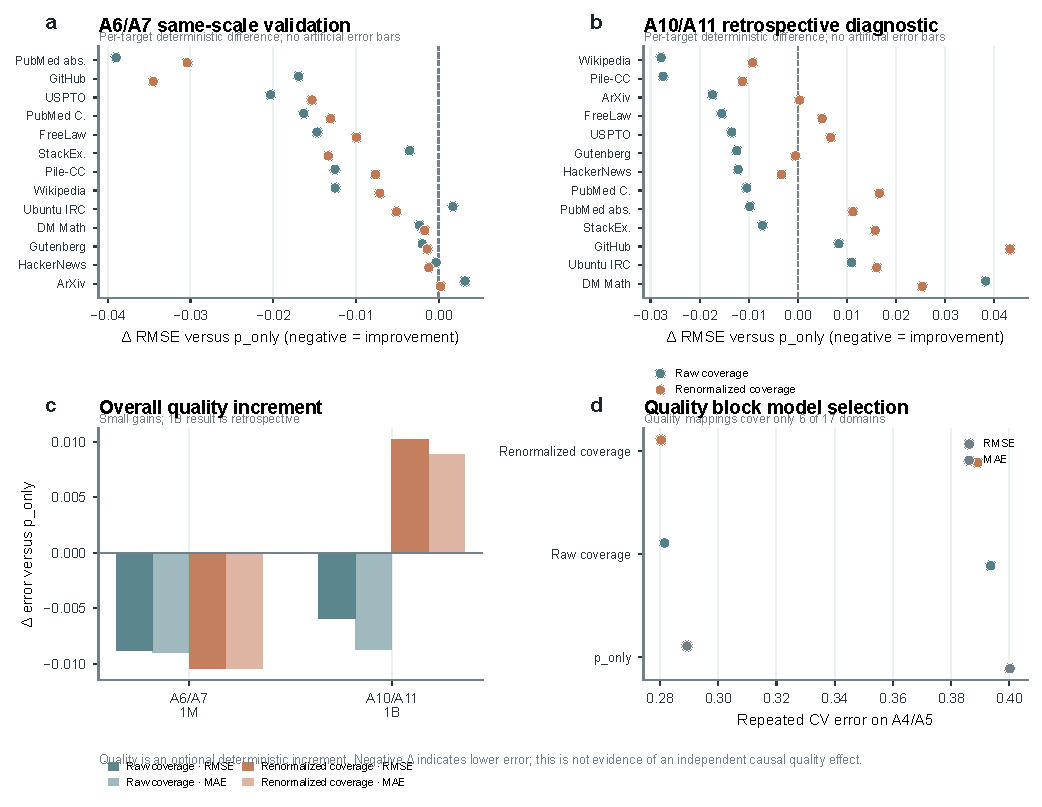
\includegraphics[width=\linewidth]{figures/q1-mixture-loss/Figure7_Q1_S03_quality_increment.pdf}
  \caption{可选质量增量修正。点表示相对于 p-only 模型的误差变化，负值表示误差下降；图中保留 13 个目标和不同数据角色。质量映射仅覆盖 6/17 个领域，$A_{10}/A_{11}$ 为回顾性诊断，故结果不作为独立质量因果证据。}
  \label{fig:q13-quality}
\end{figure}

图~\ref{fig:q13-quality} 中的质量增量不能与图~\ref{fig:q13-core} 的 M1/B1 历史诊断直接合并为一张模型排行榜：两者的目标聚合、质量版本和实验协议不同。正文主模型仍采用纯配比二阶 Ridge；质量特征只在需要进行工程校准或敏感性分析时作为附加情景报告。

\subsection{外推评价与适用边界}

在 $A_8/A_9$ 上，未经规模建模的纯配比模型出现明显绝对误差上升，说明 $L_j=f_j(\boldsymbol p)$ 不能独立解释跨规模变化。$A_{10}/A_{11}$ 同时改变规模和配方，适合用来检查迁移方向和残差结构，但不应被称作从未查看过的确认性检验。$A_{12}$--$A_{15}$ 的损失为题目给定估计值，且配方已在训练集出现，因此它们只能回答“当前模型对给定外推表是否自洽”，不能证明真实 10B 或 70B 模型已经被独立验证。

本节的定量关系还受到四个边界约束。第一，17 个配比只有 16 个自由度，零替换和坐标基会影响系数；第二，13 个 Loss 目标与 17 个训练域并非一一对应，缺少同名 Loss 的领域只能参与配方替代分析；第三，质量映射有 11 个未直接覆盖领域，且质量信号与配比存在确定性共线；第四，二阶模型的预测优势不等于每个交互项都具有稳定机制含义。因而，当前证据支持在声明的数据角色和规模范围内建立可预测的配比—Loss 关系，尚不支持跨所有规模的统一尺度律、因果领域效应或无约束最优配方。

\subsection{小结}

本节以单纯形约束下的 17 域配比为主变量，以 13 个交叉熵损失为多响应，建立了从 ILR 线性基线到二阶 Ridge 和浅层 GBDT 的候选模型链。二阶 Ridge 在 $A_4/A_5$ 交叉验证和 $A_6/A_7$ 同尺度外部验证中均取得当前候选集最小的 pooled RMSE/MAE。配对分析表明规模差异必须与配方迁移分开处理：$A_6/A_8$ 的低规模下降不能直接转移到 $A_{12}/A_{14}$ 的高规模区间。质量分支在同尺度验证中带来有限的 RMSE/MAE 降幅，但由于映射覆盖不完整且是配比的确定性函数，只作为可选增量保留。由此，问题一第三问的主结论是“配比—Loss 的可预测关系在同尺度上成立，跨尺度外推需要显式的规模与迁移边界”，而不是把任一质量或规模修正系数当作普适规律。
